\subsection{Clean Install} CJDT is
installed using the Eclipse Update Manager. We recommend you use Eclipse 3.0.\\
\subsubsection{} If you need to use a proxy server to access the internet, the first thing
to do is configure the proxy details so that the update manager can contact the
CJDT Update Site. From the Window menu select preferences, and then the
Install/Update tab.\\
\begin{figure}[htbp]
	\centering
		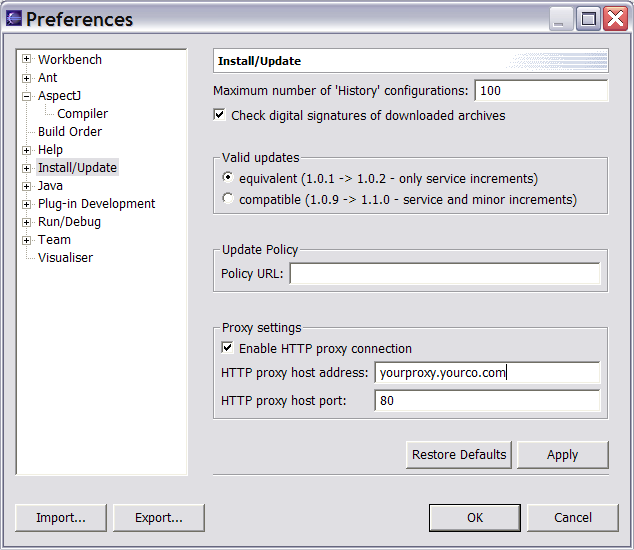
\includegraphics[width=0.85\textwidth]{./images/proxy.png}
	\label{fig:proxy}
\end{figure}
\newpage
\subsubsection{} Create an update site bookmark for the CJDT update site, and start the
install procedure.
\paragraph{In Eclipse 3.0:}
\label{sec:In Eclipse 3.0}
 From the help menu, select Software Updates -$>$ Find and Install... . Select "Search for new features to install" and click next.
Click "Add Update Site" Enter the name
"AJDT update site" \newline and the URL:  \textbf{\textit{http://download.eclipse.org/technology/ajdt/30/update}}. Click ok.\\
Fully expand the CJDT Update Site node that appears, and select "`CaesarJ"'. Click
next. Select "Eclipse CaesarJ Development Tools 0.X"\\
\begin{figure}[htbp]
	\centering
		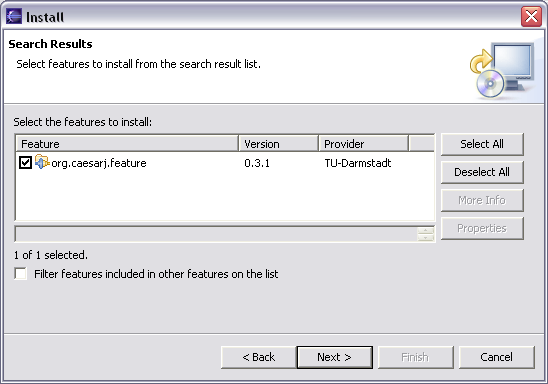
\includegraphics[width=0.85\textwidth]{./images/install_page_3_0.png}
	\label{fig:install_page_3_0}
\end{figure}\\
Select Next, accept the license agreement, and proceed to the
installation.

\subsection{Updating an Existing Installation}
Proceed as for a clean install, except that the CJDT Update Site bookmark should already
exist -- so all you need to do is expand it and go. If the version you have
installed is the same as the version on the update site (or more recent even),
then you will not be presented with any install options.
\newpage
\subsection{Is Everything OK?} 
In Eclipse 3.0 the CJDT welcome pages have been integrated into the Eclipse Platform welcome pages. You can view
these by selecting "Welcome" from the help menu and then following the Overview, Tutorials,
Samples or the What's New links.\\
\begin{figure}[htbp]
	\centering
		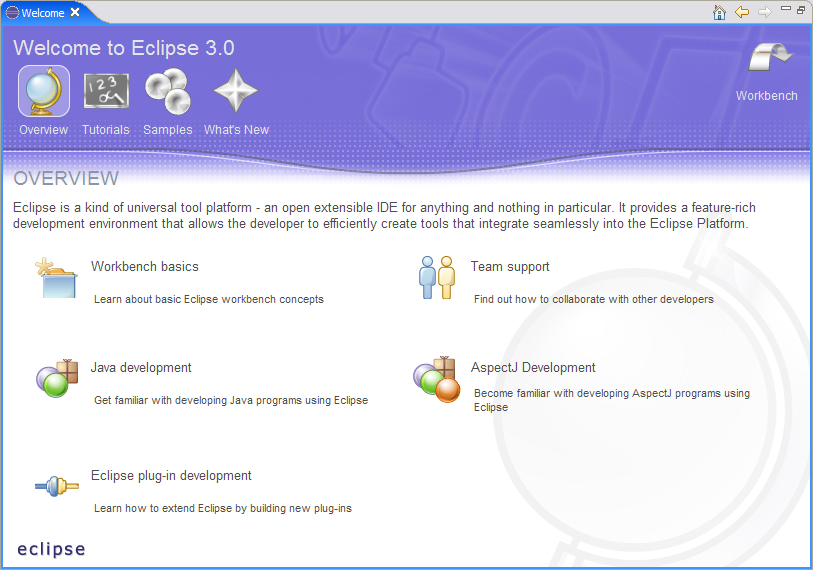
\includegraphics[width=0.95\textwidth]{./images/welcome_3_0.png}
	\label{fig:welcome_3_0}
\end{figure}
